
% ------------------------------------------------------------------------------
% Introduction
% Set the scene:
% 1) What is this thesis ? What did we find ? 
% 2) Where are gaps in the filed and what we contributed ? 
% 3) Why is this important and why mathematical modelling is a solution ? 
%.   - main parameters considered and prelude to main assumptions of the model.
% 4) The thesis summary, highlight key findings and where we sit in the field ? 
%.   - what the thesis entails and the general story line.
% -----------------------------------------------------------------------------
\chapter{Introduction}

% \begin{itemize}
%     \item talk about various routes to understanding tree disease Fig 2 of \cite{pub.1012384986} \cite{francl2001disease}
%     \item reference the applications of a model, predict the epidemic, predict control measures, crop loss, invasion and persistence, the risk of disease etc..
%     \item \cite{disease-biodiversity} disease key in biodiversity..., \cite{JOHNSON2002129} importance for landscape integrity
%     \item \cite{kelly2002monitoring} technology and capturing data via satellite. RS application \cite{doi:10.1094/PHYTO.2003.93.12.1524} \cite{doi:10.1080/0143116031000139926}
%     \item \cite{doi:10.1046/j.1523-1739.1994.08010256.x} fragmentation reference...
%     \item insects and pests intelligently seek out hosts, spores and fungicides occur passively, \textcolor{red}{double check}
%     \item talk about local infection and resolution of the problem, e.g. complicated biology of the pathogen vs dispersal distance
%     \item talk about the host-pathogen-environment dynamic \cite{pub.1012384986} Fig 3, how we are concentrating on the modelling perspective.
%     \item reference the scale problem \cite{van1999pandemics} only used small amounts of detail for large scale spread
% \end{itemize}

Modernity has witnessed drastic increases in the severity of tree disease epidemics. 
The recent development of international trade, climate change, and monocultures have increased the risk of large-scale
outbreaks in native plant and tree populations. This introductory chapter informs the reader about the importance, policy,
and modelling of infectious tree disease epidemics.

First, the motivation for studying tree disease epidemics is highlighted, 
following a review on the critical drivers of tree disease epidemics. 
Then, the challenge of evaluating epidemic control strategies, and the subsequent implementation from policymakers, is surveyed.
This Thesis will focus on the mathematical and computational modelling of tree-based epidemics in Great Britain (GB).

\newpage

\section{Invasive tree diseases}

The modern world relies heavily on imports and exports characterised by global trade networks. 
Unfortunately, importing and exporting foreign plant material can introduce invasive pests and pathogens
into non-native landscapes. Consequently, this poses worldwide risks to crops, flowering plants
and trees that may lack evolutionary defences to invasive species. \cite{doi:10.1002/9781444329988.ch8}. 

Epidemics through plant populations can be devastating.
Classic examples include Irish potato blight, Dutch elm disease \cite{doi:10.1111/j.1365-3059.2010.02391.x} 
and North American chestnut blight \cite{doi:10.1002/9780470535486.ch7}.
Two epidemics currently underway in the UK include ash dieback (Hymenoscyphus fraxineus) affecting European ash trees (Fraxinus excelsior)
\cite{ash-dieback-costs}, and Phytophthora ramorum, a prevalent disease that affects over 150 plant species, including oak, 
larch, and sweet chestnut \cite{p.ramourum}.

Trees play a pivotal role in terrestrial ecosystems \cite{boyd2013consequence}, 
and ensuring tree health marks a pressing challenge for society.
The most widely known and well-researched motivates for studying tree disease epidemics include economic,
climatic and ecological function \cite{ash-dieback-costs, freer2017tree, boyd2013consequence, tyrvainen2005benefits}. 
In particular, policymakers can execute a variety of strategies to impede the spread of disease 
to meet this complicated challenge \cite{pests-intro, Gilligan-disease-management}. 
Thinning host densities \cite{resiliency-density-reductions} or planting genetically diverse configurations
\cite{doi:10.1094/PD-89-0969, genetic-heterogeneity, huang1980importance} have been shown to increase
pathogen resilience. 

% - The progression of an epidemic can be briefly summarised by the time-line of, arrival, spread, impact and management.
% \textcolor{blue}{Expand this to include some numbers on cost and societal effects. Go into more examples of how tree diseases can cause harm to ecosystems and expand on wider environmental impacts e.g. Carbon sequestration, soil bindings and biodiversity. Expand  on current threats. !!! Talk about biology of pathogens and main divisions of diseases !!!}

% \begin{itemize}
%     \item \textcolor{red}{I could expand on the economics, along with climatic and ecological importance of trees}
% \end{itemize}

% Trees grow naturally, in both rural and urban settings, this includes commercially managed plantations and orchards. 
% Protecting and ensuring tree-health is of essential importance for society \cite{Boyd1235773}. 

% \begin{table}
%     \centering
%     \begin{tabular}{|p{3cm}||p{13cm}| }
%     \hline
%     \textbf{Benefit}&\multicolumn{1}{c|}{}\\
%     \hline
%     Social  & Recreational activities, mental and physical health, cultural and historic sentiment.\\
%     \hline
%      Aesthetic & Landscape variation, textures, colours. Seasonal dynamics which change landscape views. \\
%     \hline
%      Climatic &  Cooling, wind control, impacts on urban climate through temperature and humidity control. Air pollution reduction, sound control, glare and reflection on reduction, flood prevention and erosion control. \\
%     \hline
%      Ecological & Biodiversity and biotopes for flora and fauna.\\
%     \hline
%      Economic & Timber, wood pulp, fiber and food.\\
%     \hline
%     \end{tabular}
%     \caption{The benefits of tree health, based on \cite{tyrvainen2005benefits} and \cite{boyd2013consequence}}
%     \label{table:tree-health}
% \end{table}


\subsection{Tree disease drivers}

%-Talk about the different types of interactions and drivers, based on the pathogen biology and type of disease. How might one conceptualise it mathematically and what are the main factors to consider with tree diseases. Give an intuitive justification of the parameters used in the modelling work. Density infectivity and dispersal

The terms `pest' and `pathogen' denote a broad spectrum of taxonomically diverse organisms. 
Pests represent an organism that harms humans or human interests such as crops or livestock
\cite{buckle2015rodent, oerke2006crop, de1964biological}. Overwhelmingly, insects constitute the main
pest threats to tree species \cite{metcalf1994introduction}. In Great Britain (GB), Asian longhorn beetle
(ALB) \cite{haack2010managing}, and oak processionary moth OPM \cite{tomlinson2015managing} are two concerts
that currently threaten tree health.

In contrast, the term `pathogen' denotes any organism that induces disease. 
In the context of trees populations, diseases include fungi, bacteria, viruses, and oomycetes \cite{balloux2017q, Boyd1235773}. 
Currently, the oomycete \textit{Phytophthora ramorum} \cite{brasier2005phytophthora}, and Ash dieback (ADB)
caused by the fungus \textit{Hymenoscyphus fraxineus} \cite{ash-dieback-costs, mitchell2014ash} are two pathogens
that threaten tree-health in GB.

% \item \textcolor{red}{Expand on the plant-passport, how do I cite government reports ?}

The t\usepackage[]{}rade and transport of foreign plant material are widely recognised to increase the risk
of introducing pests and pathogens into non-native landscapes \cite{POTTER201761, lovett2016nonnative, roy2014increasing}.
Epidemics caused by non-native pathogens can be catastrophic to tree populations that lack immunity and genetic
resistance to the invasive species \cite{doi:10.1002/9781444329988.ch8}; this can be understood from an evolutionary perspective: 
in an environment unaltered by human transportation, tree and plant species are thought to co-evolve alongside pests and pathogens
in a gene-for-gene like arm-race \cite{flor1971current, dangl2001plant, Thrall1735}. 

However, the introduction of a foreign
pathogen can overwhelm a population that has no such immunity \cite{desprez2016evolutionary}. Two classic examples that shook
the world are: Dutch elm disease \cite{doi:10.1111/j.1365-3059.2010.02391.x} in the United Kingdom and chestnut blight
\cite{doi:10.1002/9780470535486.ch7} in North America.

% Control of tree disease
Recently, the importance of effective trade regulations for preventative epidemic control has become apparent
\cite{rodoni2009role}. The role of shipping and human transport is an essential factor that risks the introduction
of invasive pests and pathogens into vulnerable landscapes within a country. For example, the shipping of elm timber
infected with scolytid bark beetles, carrying the fungus \textit{Ophiostoma novo‐ulmi} was identified as an essential
factor in driving the Dutch elm outbreak in the United Kingdom \cite{doi:10.1111/j.1365-3059.2010.02391.x}. 

Thus, adequate border controls are an indispensable step in a nations arsenal to stop the spread of disease.
Ordinarily, preventative measures take the form of customs checks on imported and exported plant material such
as timber, crops or horticultural goods. In particular, the European Commission enacted plant passports to regulate
how growers and traders can transport plant material between countries\footnote{In light of Brexit, the UK now plans
to implement an equivalent passport} \cite{wulfert2010implementation}.

If checks and policy implementations fail, a pathogen might be introduced into the landscape and spread through natural
dispersal pathways. Alternatively, a pathogen might be transported into foreign ecosystems through atmospheric 
long distance dispersal (LDD) \cite{brown2002aerial}. In either scenario, biological control becomes necessary. 
The biological control of plant-based disease
can be achieved in numerous ways. Commonly, this involves chemical agents such as pesticides, predatory insects or planting
genetically resistant cultivars \cite{pal2006biological, baker1974biological}. 

In this thesis, we are motivated to investigate the eradication of tree-based pathogens 
where eradication generally entails the removal of infected and diseased trees through sanitation felling \cite{pietzsch2021effect}. 
In this case, the questions to be answered are A) How do we effectively identify an infected tree? B) 
Which infected trees are the best choices to fell? C) What is the risk that a large-scale epidemic will result?


\section{Modelling and policy}

% \cite{thompson2016management}  - problems associated with 'control'
% \cite{gaydos2019forecasting} -  workshop with policy makers
% \cite{jones2020modelling} - developing plant health models in conjunction with decision makers 
% \cite{tsouvalis2019post} - ash dieback politics

The benefit of controlling an epidemic should outweigh the costs of letting an outbreak spread unchecked. 
Plant disease modellers can help infer well-designed control policies that maximally reduce epidemic impact and minimise the expenditure
of resources\textemdash both natural and economic. However, achieving this in practice is problematic due to various unknowns \cite{13-challenges}.
Moreover, history gives examples of insufficient control policies which fail to halt pathogen spread. 
Prominent examples include Dutch elm disease in the late 1960s and early 1970s \cite{dutch-elm-mismanage}, 
and more recently citrus canker in Florida \cite{schubert2001meeting}.

With mathematical models we can attempt to understand what dictates the optimal control of tree diseases epidemics. 
Strategies have been explored on both smaller \cite{WEBIDEMICS, risk-potential-control} 
and larger landscapes \cite{large-scale-control2}. Current consensus on all spatial scales
agree that the scale of response must equal the scale of epidemic \cite{control-scale-matching}. In addition, 
any response must be carried out swiftly, otherwise the likelihood of successful management rapidly decreases and the cost of inaction soars.

Conventional eradication strategies involve detecting symptomatic trees and culling neighbours within a radius \cite{WEBIDEMICS}.
This is made difficult by numerous factors including the cryptic nature of tree diseases and resource constraints which may vary
over time \cite{control-theory, control-theory-application}. The naive strategy can be fine-tuned and optimised in many ways to increase
efficiency. One scheme involves ranking targets according to the risk they pose in order to prioritise culling \cite{risk-potential-control}.
Over large-scales, evidence suggests epidemics are most effectively controlled by targeting infected trees either at or ahead of
the infectious wave-front, as has been shown for sudden oak death in California \cite{large-scale-control}.


Optimal eradication complements enhanced `surveillance' and monitoring strategies, 
which also seek to optimise resource allocations. Here, the surveillance aims to detect infected individuals and infer disease incidence;
generally, this requires the collection and analysis of data on botanical epidemics \cite{surveillance-review}.
Ultimately, surveillance and monitoring comprise the last line of defence after preemptive boarder 
checks and inspections have failed to prevent the introduction of disease. 
Statistical approaches have been adopted to optimise the number of samples/surveys required to infer disease incidence accurately \cite{yamamura2016sampling}.
Additionally, optimal surveillance and monitoring strategies have been examined with logistic \cite{parnell2012estimating} 
and mechanistic \cite{risk-potential-control} epidemic models\textemdash the next Chapter offers a more in depth review on these modelling paradigms.

\begin{figure}
    \centering
    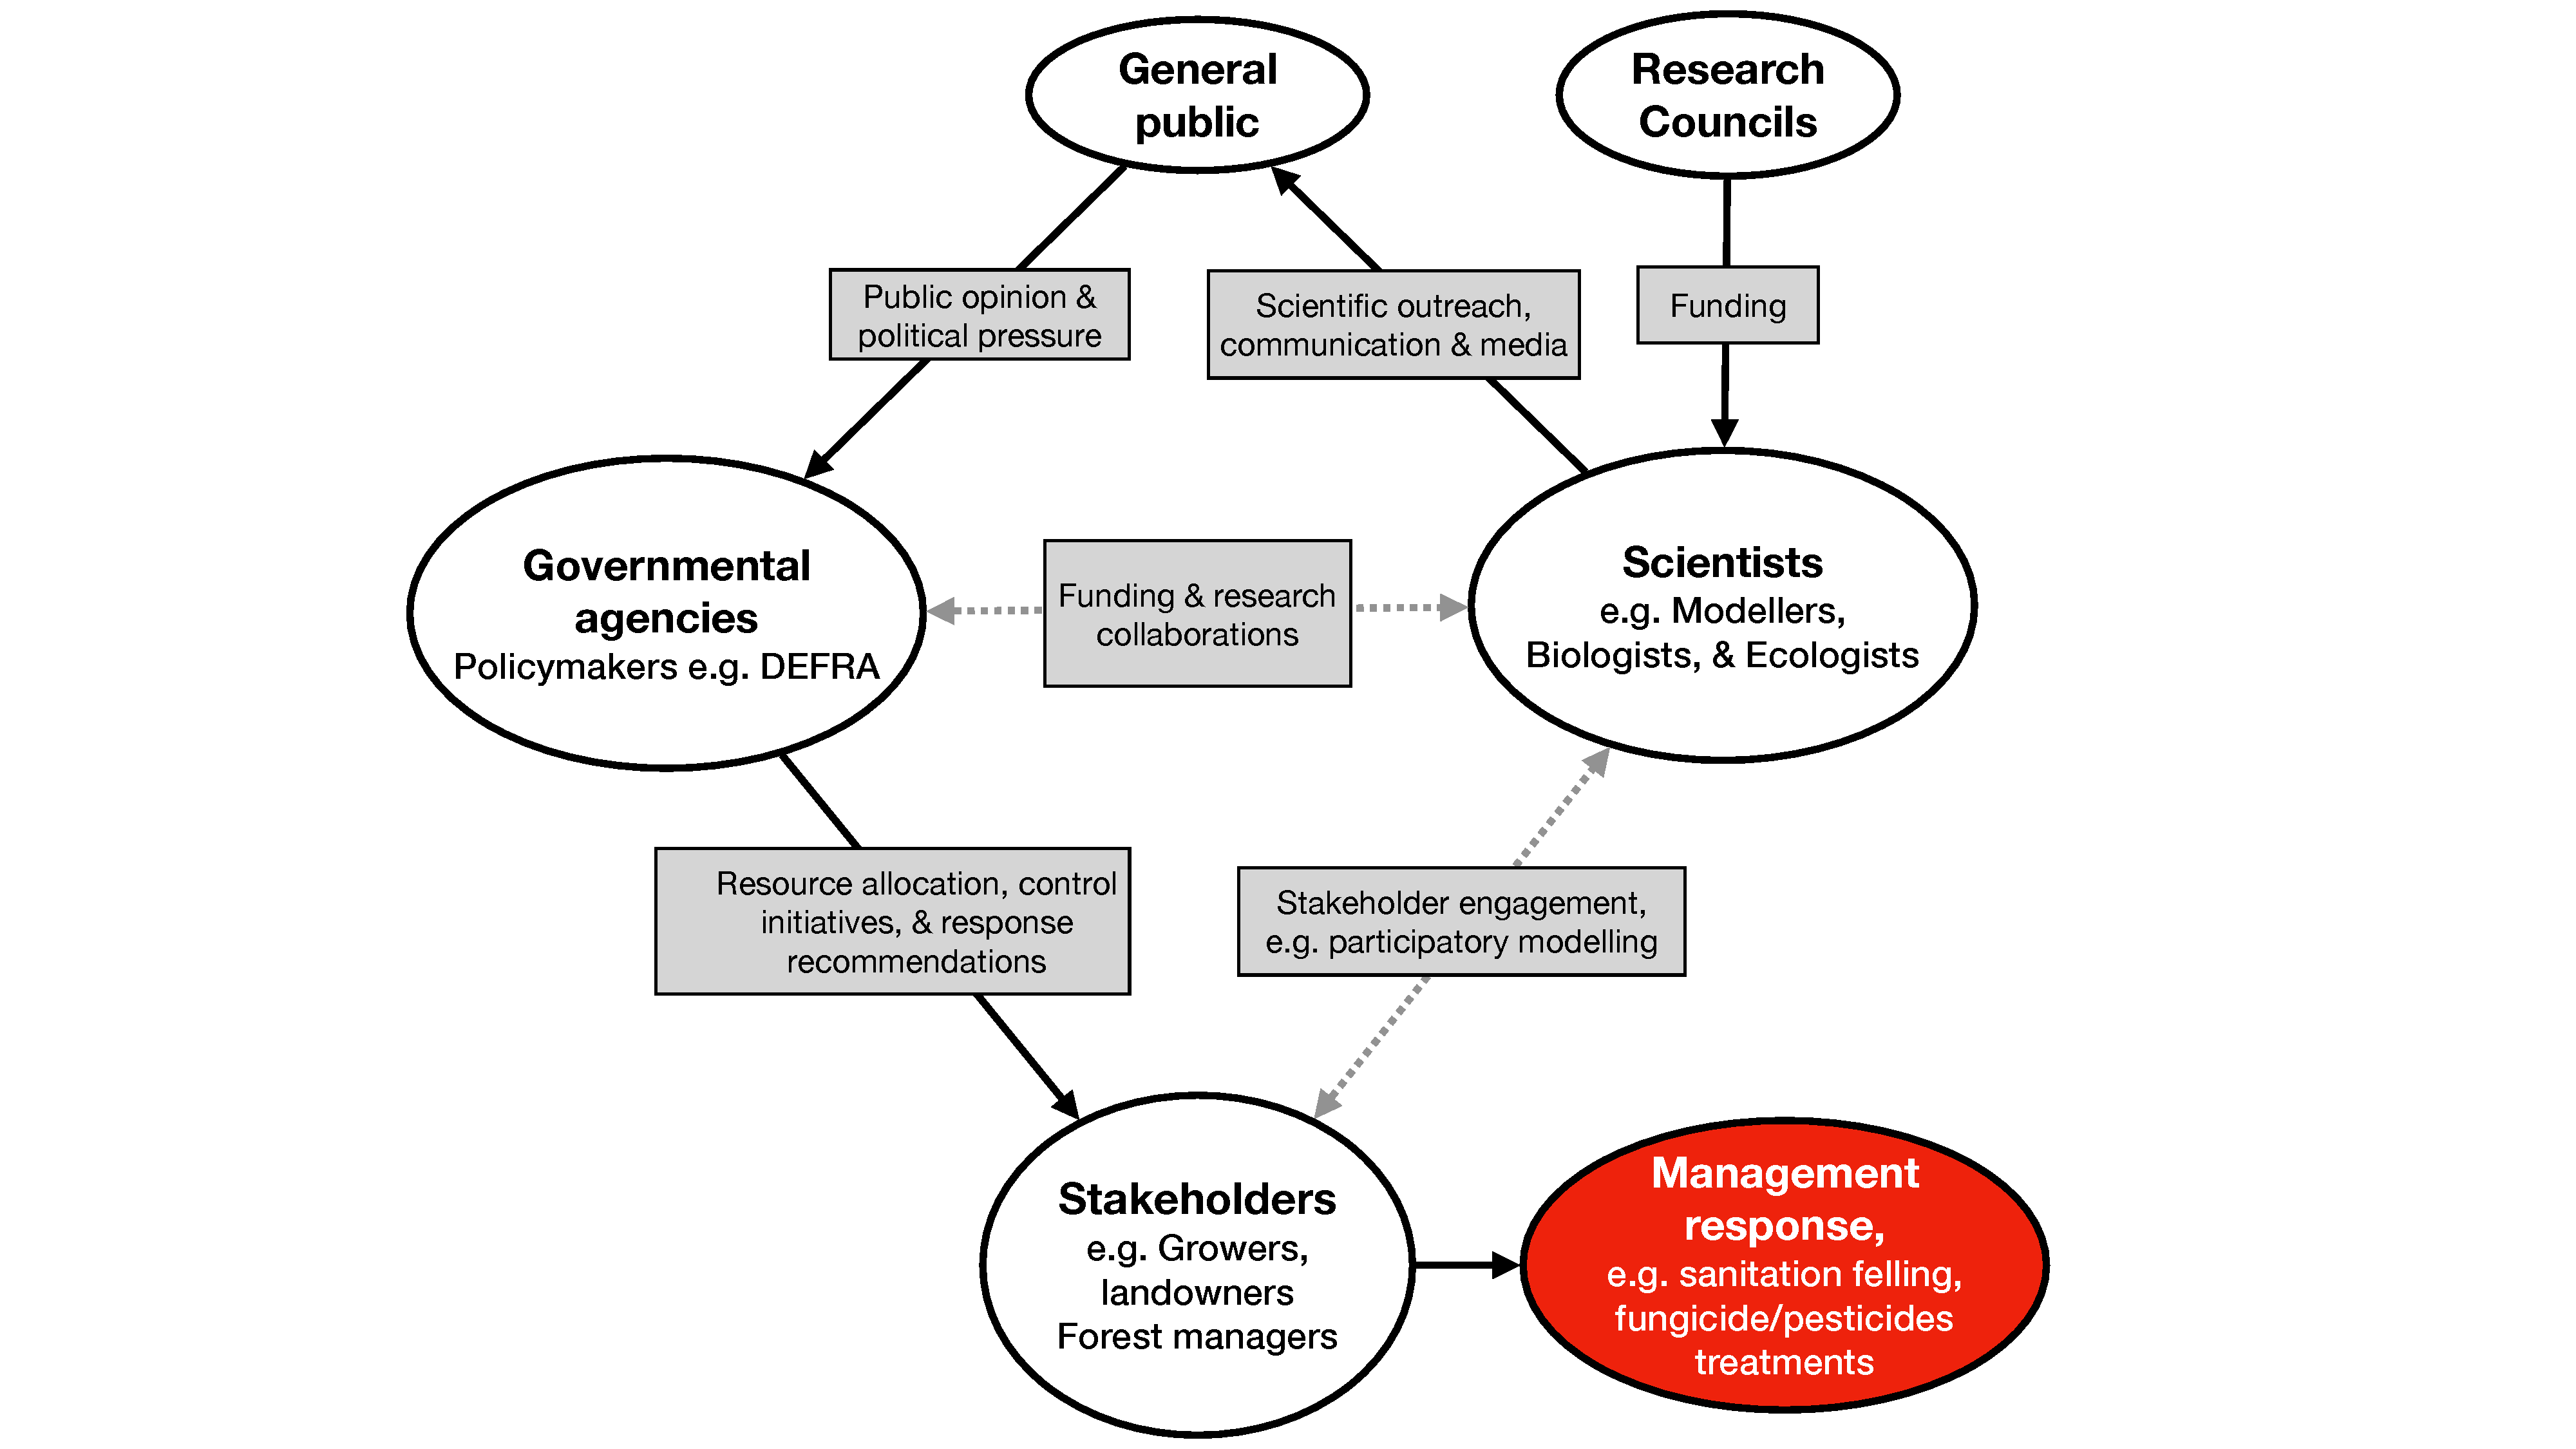
\includegraphics[scale=0.35]{chapter1/figures/modelling-and-policy.pdf}
    \caption{A (coarse-grained) model reflecting the major socioeconomic interactions between the general public, scientists, 
    policymakers and stakeholders in the UK. Scientists receive funding from and collaborate with Governmental bodies/policymakers. 
    Policymakers allocate resources and lead control initiatives to protect tree health. 
    Affected stakeholders can then join control initiatives and offer an on-the-ground response to pests and pathogens.}
    \label{fig:modelling-and-policies}
\end{figure}

Even supposing an accurate and well-informed control strategy deduced through mathematical modelling,
on-the-ground responses arise when stakeholders adopt policies or join control initiatives \cite{reed2018theory}.
Figure \ref{fig:modelling-and-policies} presents a simplified view of the interactions which dictate research output, public awareness, 
policy-making and the eventual epidemic control in the UK\footnote{Informed from informal conversations through time spent at DEFRA/Fera (San hutton, York).}.
Scientists in several disciplines\textemdash from molecular biology to mathematics\textemdash receive funding from, 
and collaborate with, governmental bodies, e.g. the Department for Environment Food \& Rural Affairs (DEFRA). 
Government led control initiatives, resource allocation and recommendations can then direct on-the-ground 
stakeholder\footnote{Here, `stakeholder' is a broad term that reflects any interested individual, collective, or organisation 
(with a stake) that have the potential to influence a policy direction or control decision \cite{brugha2000stakeholder}.
This lays in contrast to the `public' that are not directly affected by control policies and have no vested interest in the policy direction.} 
responses. 
In addition, scientists can engage stakeholders directly (discussed more below) or
influence public opinion through outreach and scientific communication. In turn, the public can influence
the decisions of policymakers through mounting sufficient political pressure \cite{fuller2016public}.

Unfortunately, several blockers inhibit a well-informed, timely and effective response. 
In particular, poor accessibility of scientific research is widely-known to inhibit policy adoption,
as disseminating scientific information requires in-depth domain knowledge and technical skill \cite{jones2020modelling}.
In a bid to make their work more accessible to policymakers and stakeholders, modellers have endeavoured construct user-friendly interfaces\footnote{
The reader can find the user-friendly modelling interface constructed by \cite{WEBIDEMICS} at \nolinkurl{http://www.webidemics.com}} \cite{WEBIDEMICS}.

Other strategies to leverage scientific output involve directly facilitating discourse between modellers and
stakeholders, categorised as `participatory modelling' (PM).
Recently, PM has become popular with risk and disaster management 
research \cite{hamalainen2020leadership, ravera2020participatory, hedelin2017participatory}.
Nonetheless, PM approaches are rare in the context of plant disease, as reviewed by \cite{gaydos2019forecasting}.

In addition to a literature review, \cite{gaydos2019forecasting} held an interactive workshop with stakeholders regarding the 
spread of \textit{P. ramorum } in the United States. The workshop facilitated stakeholder engagement with an epidemic
model \cite{tonini2017tangible} (reviewed in the preceding Chapter). In particular, the authors reported that the stakeholders
engaged well the modelling framework and confirmed that the results were realistic. However, and most interestingly, 
most of the stakeholders with expert knowledge of the landscape remained skeptical of the host distributions accuracy. 
Such insights are hard to deduce for modellers who generally remain less connected to the real landscape. 
As such, \cite{tonini2017tangible} demonstrated a firm and positive motivation to facilitate the collaboration between modellers and stakeholders through PM.

Moreover, stakeholder adoption of policies are thought to depend on a numerous other factors. 
In their analysis, \cite{\milne2020makes} coupled an epidemic model and a stakeholder opinion dynamic model.




\section{Chapter summary}

% \begin{itemize}
%     \item Talk about the general methods and strategies favoured in this thesis. Discuss main findings and the layout of this thesis, discuss where the main results fit in i.e. control of diseases.
% \end{itemize}

Here, our motivation is to develop robust models of infectious tree disease epidemics from first principles,
from which, more realistic and elaborate models can be constructed to categorise epidemic severity over GB.
Previous large-scale investigations have focused on specific pathosystems in a dynamic \textit{metapopulation-like} 
setting \cite{large-scale-control, meentemeyer2011epidemiological, harwood2009epidemiological}.
In this thesis, we take an alternative approach and develop a general-purpose framework to spatially-scale a
small-scale epidemic model (between individual trees) over large areas. The result is an $R_0$-map across GB with closer parallels 
to the emerging field of Infectious Disease Cartography \cite{otieno2021modeling, KRAEMER201619, messina2016mapping}.

Chapter \ref{chapter2:litreview} describes several key modelling themes. First, the review recounts
several seminal works that founded the field of quantitative botanical epidemiology. Following this,
a suite of small, large and multi-scale spatial epidemic models are reviewed. Additionally,
the Chapter provides an account of host distribution datasets available in GB. Lastly, a case study of the emerging
ash dieback epidemic is presented.

Chapter \ref{chapter:SLM} examines a percolation-based simple lattice model of tree disease spreading through a highly
dense forest \cite{OROZCOFUENTES201912}. The model is compartmentalised into an $SIR$ framework and 
demonstrated to exhibit a sharp threshold of transition, above which, an epidemic will propagate. 
Above the threshold of transition, a travelling wave-like behaviour is demonstrated.

Chapter \ref{chapter:SLM-applications} builds on the percolation-based model constructed in Chapter \ref{chapter:SLM}.
Firstly, we extend the work of \cite{OROZCOFUENTES201912} and present an alternative method to detect an early 
warning signal in a two-dimensional parameter space. Lastly, the epidemic model is coupled to a map of 
predicted oak abundance over GB \cite{hill.data} to outline a large-scale `toy model' of tree disease. 
Primarily, Chapter \ref{chapter:SLM-applications} demonstrates that percolation-based nearest-neighbour interactions are
problematic for realistic tree densities. 

Chapter \ref{ch5:dispersal-model} introduces a generic (non-local) Gaussian dispersal kernel into the epidemic model. 
Tree disease epidemics are demonstrated to spread at lower, more realistic tree densities and over come the inherent 
nearest-neighbour limitations witnessed in Chapter \ref{chapter:SLM-applications}. 
Disease spread is then examined over a range of dispersal scale parameters and compared to the standard $SIR$ model.
Next, a spatially-explicit analytic expression for $R_0$ is derived and compared to a `\textit{contact tracing}' method of calculating $R_0$.
Both methods of determining the reproductive ratio are shown to demonstrate a threshold at $R_0=1$.

Chapter \ref{ch:6-adb} builds on the generic (stochastic) dispersal model to construct a simplified mechanistic model 
reflecting the life cycle of ash dieback. The model involves four compartments, $SEIR$, that repeat yearly according to 
the sexual reproduction of ash dieback. Having established the seasonal $SEIR$ model, a method is presented to 
construct $R_0$-maps across GB using a map of predicted ash abundance. Lastly, a connected-component-analysis algorithm is used
to visual where $R_0$-values are more highly clustered. Examining clustering in the $R_0$-map reveals behaviour
akin to a global epidemic phase transition. That is, below a certain infectivity threshold, the pathogen would not be able to invade GB.

Building on observations discussed in Chapter \ref{ch:6-adb}, Chapter \ref{ch7:landscape-level-control} presents the first steps toward a novel
landscape-level control strategy. The epidemic control strategy is based on targeting natural
pinch-points and fault lines in the spatial distribution of hosts, which, in theory, could bottleneck the epidemic spread
between at-risk regions. The Chapter ends by discussing the major assumptions in the control method, and presents a series of research questions that need 
to addressed before the landscape-level control method is sufficiently demonstrated.